%!TEX root = thesis.tex

\chapter{Deriving stellar parameters}
\label{cha:method}


\section{Different methods for atmospheric parameters}

\subsection{IRFM}

\subsection{Photometry}

\subsection{Spectroscopy}


\section{Other stellar parameters}

\subsection{Asteroseismology}


\section{\FASMA}
\label{sec:parameters}

In this section, the process from a spectrum to atmospheric parameters will be
explained in details. There are two classic methods, synthetic fitting and
curve-of-growth analysis.

The synthetic fitting method is in simple terms a comparison between the
observed spectrum and a synthetic spectrum, which is either calculated on the
fly like SME \citep{Valenti1996}, or using a pre-calculated grid. By analysing
the $\chi^2$ the synthetic spectrum that best match the observed spectrum can be
found. This technique works for all ranges of spectral resolutions and can work
for many rotational profiles as well \citep[see e.g.][]{Tsantaki2017}. However,
this method is often time-consuming compared to the curve-of-growth analysis.

Here the curve-of-growth analysis will be explained in detail. In particular
Fast Analysis of Spectra Made Automatically (\FASMA) which was developed during
this thesis. \FASMA is made of three \emph{drivers}, 1) EW measurement driver,
2) stellar atmospheric parameters driver, and 3) abundance driver. An additional
driver is under development; a synthetic fitting driver \citep{Tsantaki2017}.
\FASMA has been made available to the community via a web
application\footnote{\url{http://www.iastro.pt/fasma/}} \citep{Andreasen2017a}.


\subsection{Ingredients}

\FASMA is written in the Python programming language and glue together other
software and models necessary for obtaining stellar atmospheric parameters from
high quality spectra. These software and models are described in greater detail
in the following sections. In short, the curve-of-growth analysis require
measured EWs where the latest version of \ARES is used \citep{Sousa2015a}. These
EWs are used to derive line abundances using model atmosphere like the ATLAS9
\citep{Kurucz1993}, MARCS models \citep{Gustafson2008}, and PHOENIX models
\citep{Husser2013} to mention the most popular for this analysis. Note that the
PHOENIX models are relative new and not as widely used yet. In tandem with model
atmospheres a radiative transfer code is also needed. \FASMA uses \MOOG
\citep{Sneden1973} for this, however there are other codes available, e.g.
\unfinished{Mention some other codes here}. The model atmosphere usually comes
in a pre-calculated grid in the $\{T_\mathrm{eff},\,\log
g,\,[\ion{Fe}/\ion{H}]\}$ parameter space. These are interpolated in order to
access the requested combination of parameters. Last, \FASMA consist of a
minimization routine which looks for the right parameters given a spectrum.



\subsection{Wrapper for \ARES}
\label{sec:measureEW}

There are two ways to measure the EW of an absorption line, manual or automatic.
Both of these methods are used here. There are advantages and disadvantages for
both method. For the manual, an advantage is that we can inspect the lines and
try to measure lines in different ways (which is useful if it is blended). We
have more control over how blended lines are fitted, and which profiles are
used. Disadvantages are that it is very time consuming, and it is prone to
errors, as a measurement might change drastically by the eyes measuring it. Even
for the same person, the measurement can change. By mentioning the advantages
and disadvantages of the manual method, it should be clear that the advantages
and disadvantages of the automatic method is the opposite of those. Especially
the time to measure the lines are orders of magnitudes faster, which is crucial
when dealing with more than a handful of spectra.

When a line is measurement by hand (manually) it is in this thesis done using
the splot command in IRAF. Here the deblending mode is used whenever necessary.
It is often necessary to fit one spectral lines with several Gaussians, as
neighbouring lines might contaminate the line of interest slightly.

When a line is measurement automatically it is in this thesis done with \ARES
\citep{Sousa2007,Sousa2015a}. When using \ARES it is important to use a correct
value of the \code{rejt} parameter. This parameter is used for placing the
continuum level, and is thus directly related to the final measurement EW. It is
difficult to get this parameter right, however the newest version of \ARES has
the option to analyse a few absorption free regions and measure the S/N. The
\code{rejt} is then calculated as:
\begin{align*}
  \mathtt{rejt} = 1 - \frac{1}{\mathrm{S/N}}.
\end{align*}

\ARES is used via the first driver of \FASMA. All the options available for
\ARES can be accessed by \FASMA. The options are setting the spectral window,
$\lambda_\mathrm{min}$ and $\lambda_\mathrm{max}$, the RV correction to be
applied or a mask to measure the RV and automatic make this correction, the
minimum and maximum EW to be considered ($\SI{5}{m}$\AA{} and $\SI{150}{m}$\AA{}
respectively), the minimum distance between two consecutive lines, the smoothing
applied with a \emph{boxcar} filter before measuring the EWs. An in-depth
description of these options can be found in \citet{Sousa2007,Sousa2015a}.

Sometimes \ARES crash when measuring an absorption line. The reason is not
clear, however when dealing with a large amount of spectra, it is important that
the analysis moves on. To deal with this problem, \FASMA finds the last line
which \ARES tried to measure in the log file. This line is temporarily removed
from the line list and \ARES is restarted. The line list used for deriving
parameters consists of numerous iron lines, thus removing one line will have a
negligible effect on the final derived parameters.



\subsection{Interpolation of atmosphere models}
\label{sec:interpolation}

\FASMA has access to both ATLAS9 models by \citet{Kurucz1993} and MARCS models
by \citet{Gustafson2008}, both are in a pre-calculated grid as described above.
Let this grid be described by $\{T_\mathrm{eff,g},\,\log
g_g,\,[\ion{Fe}/\ion{H}]_g\}$, where $g$ is one of the grid points. Such a grid
can be seen in \fref{fig:grid} for $[\ion{Fe}/\ion{H}]=0.00$ in the
$T_\mathrm{eff}$ range; $\SIrange{3000}{10000}{K}$. For visualisation the
location of the Sun is shown as well. The colour scale corresponds to the
temperature in the first layer of each model atmosphere, i.e. the uppermost
layer. The requested value will be $\{T_\mathrm{eff,r},\,\log
g_r,\,[\ion{Fe}/\ion{H}]_r\}$. The task is now to find the surrounding grid
points in the parameter space of the requested parameters. For $\log g$ and
$[\ion{Fe}/\ion{H}]$ two neighbouring grid point are used, and for
$T_\mathrm{eff}$ four surrounding grid point are used, in total
$4\times2\times2=16$ model atmospheres for the interpolation. \FASMA use the
four surrounding grid points for $T_\mathrm{eff}$ instead of two, since the
model atmosphere changes most with $T_\mathrm{eff}$. This is common in other
interpolations\reference{Give ref here} as well.

\begin{figure}[htpb!]
    \centering
    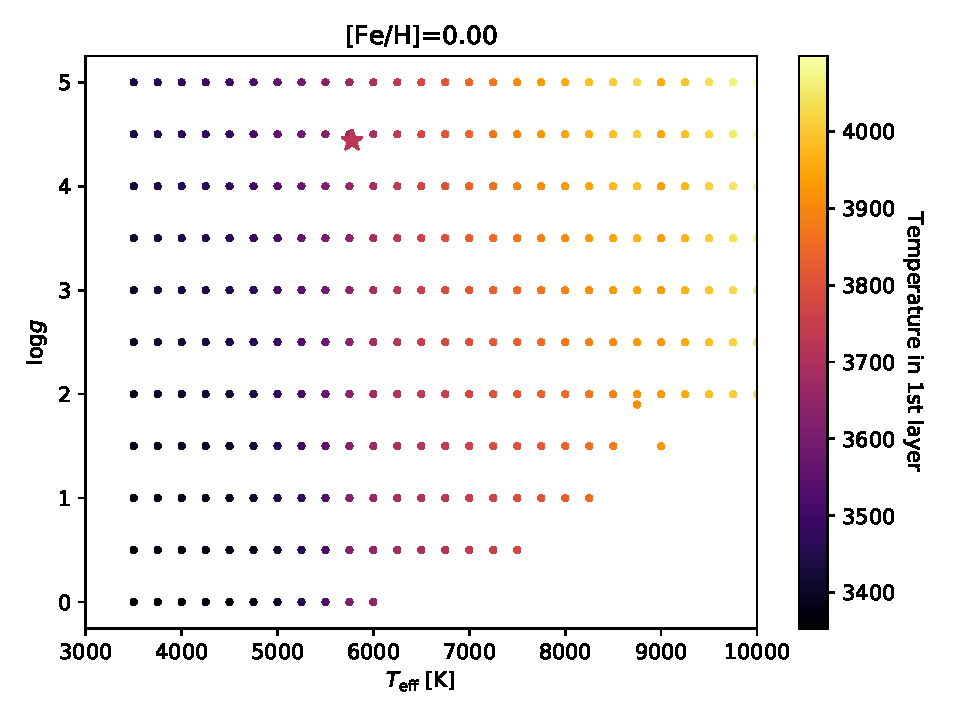
\includegraphics[width=1.0\linewidth]{figures/model_atmosphere.pdf}
    \caption{Model atmosphere grid from \citet{Kurucz1993} at
             $[\ion{Fe}/\ion{H}]=0.00$ between \SI{3000}{K} and \SI{10000}{K}.
             The grid extends to higher $T_\mathrm{eff}$, but these are not
             considered in this thesis.}
    \label{fig:grid}
\end{figure}

When the 16 model atmosphere have been located, the interpolation goes through
each layer of the model atmosphere, where there typical are 72 layers, and each
column of which there are six. The columns are described in
\sref{sec:atmospheremodels}. The interpolation are done using the
\code{griddata} function from \code{SciPy}\footnote{\url{https://scipy.org/}}.
The interpolation is linear in the parameter space. After the interpolation, the
result is saved to a file in the format expected by \MOOG.






\subsection{Minimization}

\improvement{Include figures with abundance vs. EP/RW}
With the measured EWs for all the lines in the line list, we choose an
atmosphere model to determine the abundances. If there is no prior knowledge of
the star it is common simple choose a solar atmosphere model as a starting
point. Next the correlation between the abundances and the reduced EWs, and the
abundances and the excitation potential is calculated. If there is a correlation
it means the atmosphere model used is wrong. Moreover, we also have to check if
the mean abundance of \ion{Fe}{I} and \ion{Fe}{II} lines are equal, and last if
mean abundance of the \ion{Fe}{I} lines is equal to the input
$[\ion{Fe}/\ion{H}]$ of the atmosphere model\footnote{We use \ion{Fe}{I} instead
of \ion{Fe}{II} lines for this, since they are more numerous.}. If one of these
four criteria does not pass, then the atmosphere model is wrong, and we have to
search for a new one. A common way to do this, is by combining the indicators
into a scalar value:
\begin{align}
  f(\{T_\mathrm{eff}, \log g, [Fe/H], \xi_\mathrm{micro}\}) &= \sqrt{a_\mathrm{EP}^2 + a_\mathrm{RW}^2 + \Delta\ion{Fe}{}^2},
\end{align}
where $a_\mathrm{EP}$ is the correlation between abundances and excitation
potential, $a_\mathrm{RW}$ is the correlation between abundances and reduced EW,
and $\Delta\ion{Fe}{}$ is the difference between the mean abundances of
\ion{Fe}{I} and \ion{Fe}{II}. This scalar function can be minimized using
standard minimization procedures as the simplex downhill among others. However,
there is another approach that takes into the account the information stored in
these indicators. For example, if $a_\mathrm{EP}$ is positive it means
$T_\mathrm{eff}$ has to be increased by an amount correlated by the numerical
value of $a_\mathrm{EP}$. In the same way, a non-zero $a_\mathrm{RW}$ means
$\xi_\mathrm{micro}$ has to be changed, and $\Delta\ion{Fe}{}$ is an indicator
for $\log g$. In the end it is a vector function being minimized which are more
difficult, however we are not minimizing this using standard mathematical
methods, but rather using the physical knowledge. This minimization is useless
for anything else, but it is excellent for this.
The vector function has the form:
\begin{align}
    f(\{T_\mathrm{eff}, \log g, [Fe/H], \xi_\mathrm{micro}\}) = \{a_\mathrm{EP}, a_\mathrm{RW}, \Delta\ion{Fe}, \ion{Fe}{I}\}.
\end{align}

In each iteration where convergence is not reached, the input metallicity is
changed to that of the mean output metallicity using the \ion{Fe}{I} lines. The
minimization is depicted in \fref{fig:minimization}. This minimization is
written in the Python programming language and is also a wrapper around both
\ARES and \MOOG. The entire package is called \FASMA\footnote{Greek for
spectrum} \citep{Andreasen2017a, Tsantaki2017}. \FASMA is able to fix one or all
of the four atmospheric parameters, and when it reach convergence it checks if
there are any outliers in the abundances. These will be removed, either all at
once, all iteratively, meaning that after removing the outliers the minimization
is restarted at the previous best parameters, and this process is continued
until there can be removed no other outliers, or last is removing one outlier
iteratively. An optical line list like the ones by
\citet{Sousa2008a,Tsantaki2013} have been tested thoroughly and it is safe to
remove a larger amount of lines and still obtain reliable parameters. However,
with a less tested line list, like the one by \citet{Andreasen2016} (and refined
in \citet{Andreasen2017b}), one should remove outliers more carefully, and it is
recommended that one outlier is removed iteratively.

In \fref{fig:minimization} there is a flag with \emph{autofixvt}. This was an
option introduced since we see that some spectra does not converge, however the
usual way to proceed is to fix the $\xi_\mathrm{micro}$. This is done at the end
of the minimization if the $\xi_\mathrm{micro}$ value is close to either
$0\si{km/s}$ or $5\si{km/s}$ and $|a_\mathrm{RW}| > 0.050$. When fixing
$\xi_\mathrm{micro}$ with \FASMA, its value is changed in each iteration
following a simple empirical relation:
\begin{align}
  vt = \begin{cases}
    6.935 \cdot 10^{-4}\; T_\mathrm{teff} - 0.348 \log g - 1.437     & \text{For $\log g \ge 3.95$} \\
    2.72 - 0.457 \log g + 0.072 \cdot [\ion{Fe}/\ion{H}]             & \text{For $\log g < 3.95$},
\end{cases}
\end{align}
where the first case is from \citet{Tsantaki2013} and the latter case is from
\citet{Adibekyan2015}.

Last there is an option, \emph{refine}. This apply more strict criteria for the
indicators to reach convergence, thus making the minimization less sensitive to
the initial guess since it could otherwise reach convergence from one "side" of
the parameter space. The default criteria are:
\begin{align*}
  a_\mathrm{EP}     &= 0.001\\
  a_\mathrm{RW}     &= 0.003\\
  \Delta\mathrm{Fe} &= 0.001.
\end{align*}
The criteria for $a_\mathrm{RW}$ is not as strict as $a_\mathrm{EP}$ since this
indicator can change rapidly with small changes in $\xi_\mathrm{micro}$, thus a
very strict criteria might never lead to convergence. Convergence is reached
once all of the above criteria are met, and the input and output metallicity are
identical. If one or more of the parameters are fixed, the corresponding
criterion is simply set to 0 and effectively ignored, thus not changing the
parameter.

For each iteration, the change to be applied for the atmospheric parameters are
defined by adding the following:
\begin{align}
  T_\mathrm{eff}     &: \SI{2000}{K} \cdot a_\mathrm{EP}   \\
  \xi_\mathrm{micro} &: \SI{1.5}{km/s} \cdot a_\mathrm{RW} \\
  \log g             &: -\Delta\mathrm{Fe}
\end{align}
to each parameter. Note again that metallicity is simply changed to the the
output metallicity of the previous iteration. These are empirical relations.
Note that by changing e.g. $T_\mathrm{eff}$ not only is $a_\mathrm{EP}$
affected, but the other indicators as well. So there is a inter-dependency
between the parameters, however this is ignored by \FASMA as it is not a simple
problem to solve. The stepping presented above is chosen to rapidly reach
convergence, without causing problems for the inter-dependency.

\begin{figure}[htpb!]
    \centering
    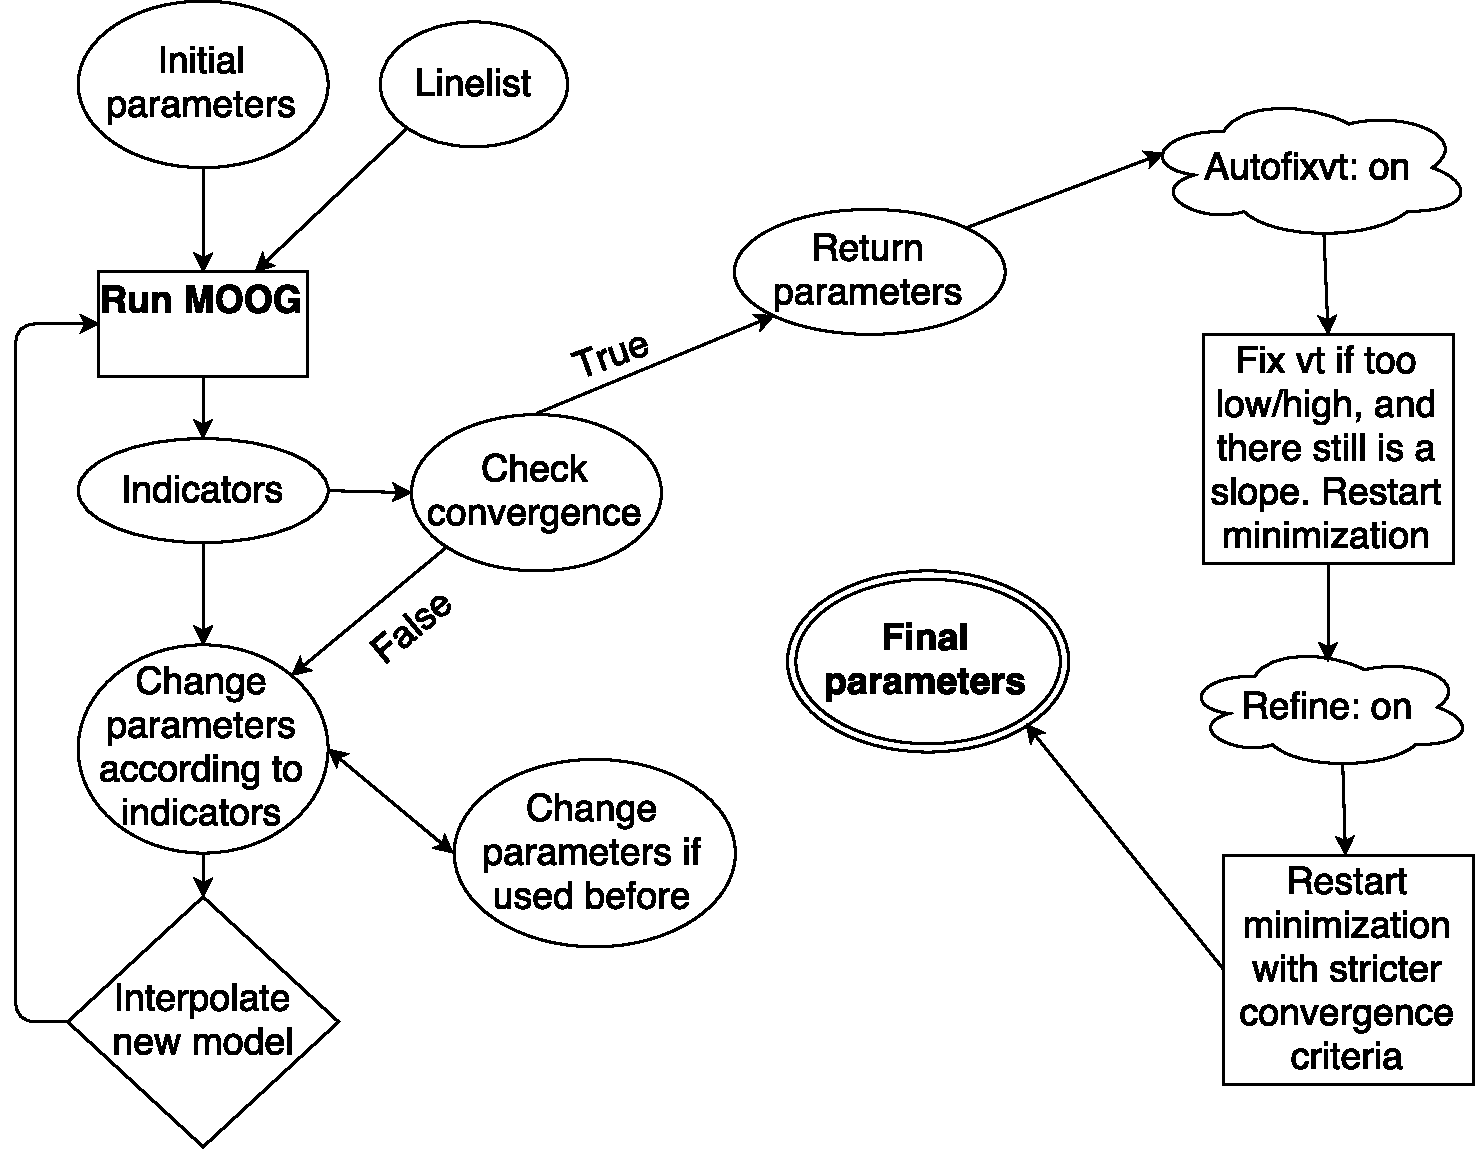
\includegraphics[width=1.0\linewidth]{figures/FASMA_minimization.pdf}
    \caption{Overview of the minimization for \FASMA. Credit: \citet{Andreasen2017a}.}
    \label{fig:minimization}
\end{figure}

\subsection{Error estimate}
